\documentclass{article}
\usepackage[utf8]{inputenc}
\usepackage{amsmath,amsfonts,amssymb}
\usepackage[margin=1in]{geometry}
\usepackage[parfill]{parskip}
\usepackage{authblk} % Better formatting of affiliations.
\usepackage{graphicx} % Allow graphics
\usepackage{xcolor} % Allow colored text.
\usepackage[sort&compress]{natbib} % Better bibliography formatting

% for nice url formatting, including auto linebreaks
\usepackage{xurl}

% makes nice looking tables
\usepackage{tabularx}

% get periods in figure captions instead of colons
\usepackage[labelsep=period]{caption}

% indicate FIXMEs with red text
\newcommand{\fixme}[1]{{\color{red}{#1}}}

% get 'Abstract' in all caps. This is a bit hacky
\renewcommand\abstractname{\textsc{ABSTRACT}}

% enable superscript in-text citations
\usepackage[superscript]{cite}

\title{Evaluating proteomics imputation methods with improved criteria}

\author[1]{Lincoln Harris}
\author[2]{William E.\ Fondrie}
\author[3]{Sewoong Oh}
\author[1,3,*]{William S.\ Noble}

\affil[1]{Department of Genome Sciences, University of Washington,  Seattle, Washington, 98195, United States}
\affil[2]{Talus Biosciences, Seattle, Washington, 98112, United States}
\affil[3]{Paul G.\ Allen School of Computer Science and Engineering,
  University of Washington, Seattle, Washington, 98195, United States}
\affil[*]{Corresponding author. Email: william-noble@uw.edu}

\date{}

\begin{document}

\maketitle

\begin{abstract}
Quantitative measurements produced by tandem mass spectrometry proteomics experiments typically contain a large proportion of missing values. Missing values hinder reproducibility, reduce statistical power, and make it difficult to compare across samples or experiments. Although many methods exist for imputing missing values, in practice, the most commonly used methods are among the worst performing. Furthermore, previous benchmarking studies have focused on relatively simple measurements of error, such as the mean-squared error between imputed and held-out values.  Here we evaluate the performance of commonly used imputation methods using three  practical, ``downstream-centric'' criteria. These criteria measure ability to identify differentially expressed peptides, generate new quantitative peptides, and improve peptide lower limit of quantification. Our evaluation comprises several experiment types and acquisition strategies, including data-dependent and data-independent acquisition. We find that imputation does not necessarily improve the ability to identify differentially expressed peptides, but that it can identify new quantitative peptides and improve peptide lower limit of quantification. We find that MissForest is generally the best performing method per our downstream-centric criteria. We also argue that existing imputation methods do not properly account for the variance of peptide quantifications and highlight the need for methods that do.
\end{abstract}

\textbf{KEYWORDS:}
\textit{Quantitative mass spectrometry, proteomics, imputation, machine learning, statistics, differential expression, lower limit of quantification}

\section{INTRODUCTION}

The quantitative accuracy and sensitivity of tandem mass spectrometry proteomics has increased dramatically in the past decade. In spite of this trend, proteomics experiments are still limited by excessive ``missingness,'' which refers to peptides that are present in the sample matrix but are not assigned an abundance value. Missingness can be attributed to a variety of technical factors including ion suppression, co-eluting peptides, the lower limit of quantification of the instrument, and the failure to confidently assign peptides to all observed spectra \cite{Bramer:review, Webb-Robertson:review}. Although low abundance peptides are generally more likely to be missing, peptides may be missing across the entire range of intensities. Missingness decreases the statistical power of proteomics experiments, hinders reproducibility, and makes it difficult to compare across batches or experiments \cite{Bramer:review, Webb-Robertson:review}.

Imputation is a bioinformatic solution to the missingness problem. Imputation refers to using statistical or machine learning procedures to estimate missing values in a data set. While still relatively new within the proteomics community, imputation has long been standard practice for analysis of gene expression, \cite{knn-impute} clinical and epidemiological data \cite{multi-impute-clinical}, and more recently astronomy \cite{astro-impute1, astro-impute2} and single-cell transcriptomic data \cite{ALRA, magic-scRNA}. Imputation methods for proteomics data (Table~\ref{tab:method-descrip}) fall into three broad categories: ``single-value replacement'' methods, in which all missing values are filled in with a single replacement value; ``local similarity'' methods, which use statistical models to learn patterns of local similarity in the data, for example between subsets of similar peptides or runs; and ``global similarity'' methods, which learn broad patterns of similarity across all peptides and runs.

\begin{table}
  \centering
  \scriptsize
  \begin{tabular}{lcp{3in}p{1in}}
    \hline
    Method & Type & Description & Examples \\
    \hline
    Zero replacement & S & Replace missing values with zeros & \\
    Mean replacement & S & Replace missing values with the mean peptide intensity for a peptide or sample & \\
    Low value replacement & S & Replace missing values with the lowest observed intensity in any sample (sample minimum) or peptide (peptide minimum) & \\
    Gaussian random sample & S & Randomly sample from a Gaussian distribution centered around the lowest observed intensity & Perseus \cite{Perseus} \\
    Regression & L & Linear regression is used to estimate missing values & lm, glm \\
   kNN & L & Weighted average intensity of $k$ most similar peptides & impute.knn \cite{knn-impute}, VIM \cite{VIM} \\
    MissForest & G & Nonparametric method to impute missing values
using a random forest classifier trained on the observed parts of the data set,
repeated until convergence & MissForest \cite{missForest} \\
    PCA & G & Run principal component analysis, impute missing values with the regularized reconstruction formulas and repeat until convergence & pcaMethods \cite{pcaMethods}, missMDA \cite{missMDA} \\
     \hline
  \end{tabular}
  \caption{{\bf Existing proteomics imputation methods.} Descriptions of generalized imputation strategies and examples of specific tools that implement each strategy.  The ``Type'' column indicates whether the method uses single-value replacement (S), local similarity (L), or global similarity (G).
    \label{tab:method-descrip}}
\end{table}

It is not always clear what imputation method is best for a given proteomics data set. A number of studies benchmark imputation methods and offer guidelines for selecting an appropriate method \cite{Bramer:review, Webb-Robertson:review, DIMA, lazar, valikangas, dabke}. A general recommendation is that single-value replacement strategies rarely work well. Another is that the optimal imputation method depends on the structure of missingness in the data. Mass spectrometry-based proteomics experiments exhibit two major forms of missingness: missing completely at random (MCAR) and missing not at random (MNAR). MCAR describes missingness that does not depend on any observed variable, that is, missingness occurs independent of peptide intensity or relationships between samples. For MNAR, missingness \textit{is} dependent on some observed variable. For example, in mass spectrometry-based proteomics, missingness is often a function of peptide intensity, with more missingness occurring in peptides closer to the instrument's lower limit of quantification (LLOQ).

When comparing performance of imputation methods, it is commonplace to use relatively simple criteria that are easy to compute but not necessarily relevant to most proteomics researchers. One example is calculating the mean squared error (MSE) between imputed and ground truth peptides quantifications for a withheld set of matrix entries. As an alternative, we introduce ``downstream-centric,'' criteria focused on differential expression, peptide LLOQ, and the total number of quantitative peptides in an experiment. We argue that these downstream-centric criteria are more relevant to the questions proteomics researchers typically seek to answer. Furthermore, we observe that the best-performing imputation methods per traditional criteria often differ from the best performing methods per our downstream-centric criteria. 

\begin{figure}
  \begin{center}
    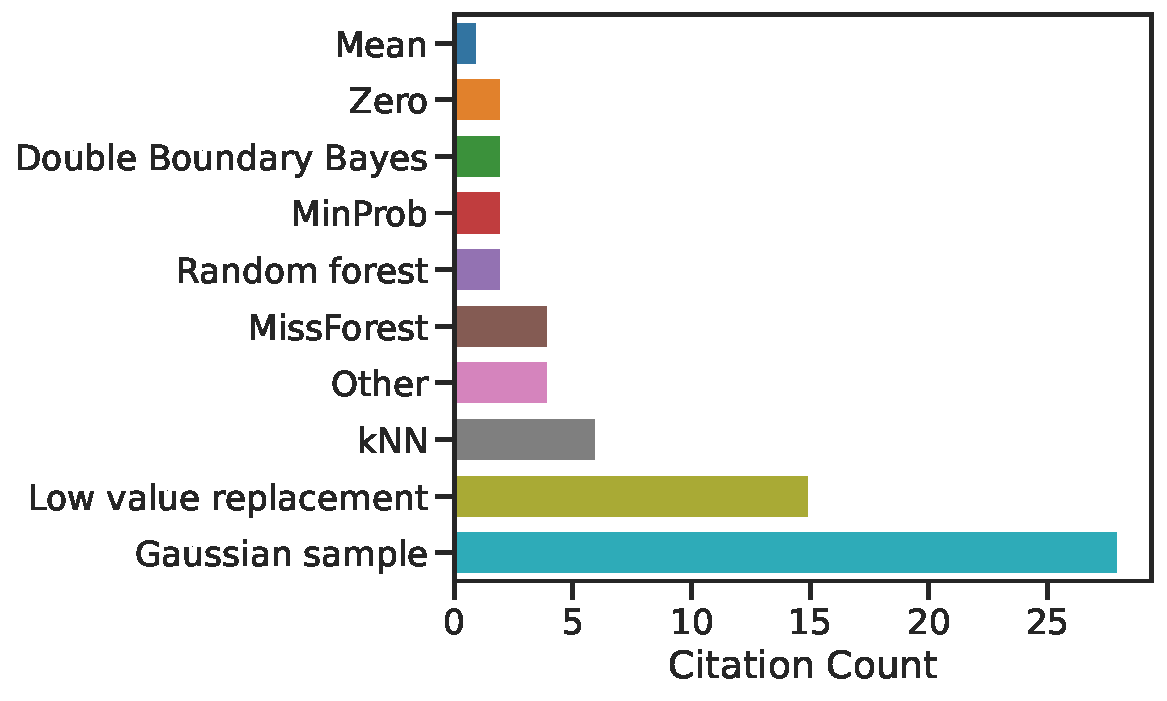
\includegraphics[width=0.6\textwidth]{figures/literature-survey-figure.pdf}
  \end{center}
  \caption{{\bf Identifying the most commonly used proteomics imputation methods.} Results of a literature survey of \textit{Journal of Proteome Research} articles from January, 2019 -- January, 2023 are shown. Methods labeled ``Other'' appear in just a single publication, and refer to the imp4p and QRLIC R packages, as well as methods based on Euclidean distances and randomly drawing from the entire peptide intensity range.  The full results of this literature search, including the names and DOIs of the identified studies, are included as Data 1.}
  \label{fig:citation-counts}
\end{figure} 

To decide which imputation methods to include in our study, we carried out a systematic literature review.  All \textit{Journal of Proteome Research} articles published between January 1, 2019, and January 31, 2023, were searched for the following terms: ``impute,'' ``imputed,'' ``imputation.'' For this survey we excluded methodological and benchmarking studies.  On the basis of the resulting citation counts (Figure~\ref{fig:citation-counts}), we selected four of the most popular imputation methods: $k$-nearest neighbor (kNN)  \cite{knn-impute}, MissForest \cite{missForest}, Gaussian sampling \cite{Perseus}, and low value replacement.   We also include a non-negative matrix factorization (NMF) imputation method, which has recently been proposed for proteomics \cite{nmf-metabolomics, ms-impute, deep-impute}.  By focusing on only the most commonly used imputation methods, our aim is to provide a practical comparison that will be beneficial to experimental proteomicists. For this reason, seldom used R packages (e.g., imp4p, impSeqRob, QRLIC) have been omitted from our analysis. We also omit PCA-based methods, as they did not come up in our literature review.

Additionally, we choose to conduct our analysis primarily on peptide-level quantifications. Our reason for this is severalfold: (i) summarizing peptide quantifications at the protein level reduces often-critical data heterogeneity \cite{humpty-dumpty}, (ii) protein roll-up can introduce statistical bias \cite{boekweg-2023}, and (iii) imputation may perform better at the peptide level \cite{lazar}.

We evaluate performance of the five imputation methods with both traditional and downstream-centric criteria. The latter include the ability to: (i) identify differentially expressed peptides, (ii) generate new quantitative peptides, and (iii) improve peptide LLOQ. Our benchmarking study comprises a variety of experiment types including serial dilution series, data-dependent acquisition (DDA), data-independent acquisition (DIA), label-free, and isobaric labeled experiments. Critically, we include an unimputed condition in all three downstream-centric evaluation experiments, for evaluating whether imputation should be performed at all. Our findings suggest that imputation may not improve detection of differentially expressed peptides, but that it can identify new quantitative peptides and improve peptide LLOQ.

We also demonstrate that the variance among measured peptide intensities is greater than expected. Ion detection is a Poisson process and quantifications from ion-counting mass spectrometers are often assumed to be Poisson distributed \cite{ms-dist-derivation, stat-theory-lcms}. We demonstrate that peptide quantifications are overdispersed relative to a Poisson model and that log transformation does not result in uniform variance. This finding demonstrates that the statistical assumptions made by several prominent imputation methods are not met in proteomics data. It also suggests the need for methods that employ variance stabilization prior to imputation, similar to strategies taken in genomics \cite{variance-stable, ZINB, neg-binom-scRNAseq}.

\section{METHODS}

\subsection{Data sets}

For this study, we used 12 public quantitative proteomics data sets (Table \ref{tab:data-description}). Eight of the 12 data sets were accessed via the Proteomics Identification Database (PRIDE, \url{https://www.ebi.ac.uk/pride/}) \cite{PRIDE}, and are indicated with their ProteomeXchange (PXD) labels \cite{ProteomeXchange}. Two data sets were obtained from the National Cancer Institute's Clinical Proteomic Tumor Analysis Consortium (CPTAC) data portal (\url{https://proteomic.datacommons.cancer.gov/pdc/}) \cite{CPTAC}.  The remaining two data sets, PXD034525 and PXD014815, were obtained from Panorama (\url{https://panoramaweb.org/home/project-begin.view}). Additional details on data set acquisition are provided by Data 2.

For experiments processed with MaxQuant, we used the ``peptides.txt'' output files to generate peptide-by-run intensity matrices by selecting only the ``Sequence'' and ``Intensity'' columns. For the CPTAC experiments, we obtained peptide-spectral match files (.psm) from the CPTAC data portal and converted them to matrix format with custom scripts (available at \url{https://github.com/Noble-Lab/2023-prot-impute-benchmark}). The peptide-by-run matrices from these CPTAC studies were large (S047: 110,000 peptides $\times$ 226 samples; S051: 291,000 peptides $\times$ 35 samples). For efficiency, we downsampled these matrices by randomly selecting 40,000 peptides and 30 runs from each. 

For the two DIA data sets, peptide quantification matrices were obtained directly from Panorama.

\begin{table}
  \centering
  \begin{tabular}{lrrrrrr}
    \hline
    Identifier & Peptides & Runs & \% Missing & Quantification Software & Experiment Type & Citation \\
    \hline
    PXD016079 & 32999 & 31 & 45 & MaxQuant, MBR & DDA, LFQ & \cite{pxd016079} \\
    PXD006109 & 38124 & 20 & 17 & MaxQuant, MBR & DDA (BoxCar) & \cite{pxd006109} \\
    PXD014525 & 17208 & 36 & 92 & MaxQuant & DDA, LFQ & \cite{pxd014525} \\
    PXD034525 & 40346 & 10 & 13 & EncyclopeDIA, Skyline & DIA & \cite{smtg-maccoss} \\
    PXD014815 & 24204 & 42 & 29 & EncyclopeDIA, Skyline & DIA & \cite{matrix-matched-calib} \\
    PXD013792 & 2224 & 12 & 72 & MaxQuant & DDA, LFQ & \cite{pxd013792} \\
    PXD014156 & 697 & 20 & 55 & MaxQuant & DDA, LFQ & \cite{pxd014156} \\
    PXD006348 & 10362 & 24 & 72 & MaxQuant & DDA, LFQ & \cite{pxd006348} \\
    PXD011961 & 23415 & 23 & 46 & MaxQuant, MBR & DDA, LFQ & \cite{pxd011961} \\
    CPTAC-S047 & 40000 & 30 & 54 & Philosopher & DDA, TMT & \cite{CPTAC-S047} \\
    CPTAC-S051 & 40000 & 30 & 41 & Spectrum Mill & DDA, TMT & \cite{CPTAC-S051} \\
    PXD007683 & 38921 & 11 & 0 & Custom pipeline & DDA, TMT & \cite{pxd007683} \\
    \hline
  \end{tabular}
  \caption{{\bf Data set characteristics.} Description of the proteomics data sets used in this study. The two CPTAC data sets were downsampled by randomly selecting 40,000 peptides and 30 runs each. ``MBR'' stands for ``match between runs,'' ``LFQ'' for ``label-free quantification,'', and ``TMT'' for ``tandem mass tag.'' References for quantification software: MaxQuant \cite{MaxQuant}, EncyclopeDIA \cite{chromatogram-DIA}, Skyline \cite{skyline}, Philosopher \cite{philosopher}.}
    \label{tab:data-description}
\end{table}

\subsection{Traditional evaluation measures}

We first used a traditional machine learning-style train/test setup to evaluate the performance of imputation methods. With this approach, the values in the peptide-by-run matrix were randomly partitioned into two groups: a training set and a test set.  The imputation method was trained on the training set values and we measured how well the method imputed the values in the test set.  For each data set, peptides with fewer than four present values in the training set were removed prior to imputation.

The train/test partitioning was performed with two different procedures: MCAR and MNAR. For MCAR, 25\% of the present (i.e., non-missing) matrix entries were randomly selected for the test set. The remaining matrix entries were used as the training set.  For MNAR, we took a similar approach to the one described by Lazar \textit{et al.} \cite{lazar}. For a given peptide-by-run matrix, we constructed an equally sized thresholds matrix filled with values sampled from a Gaussian distribution centered about the 30\textsuperscript{th} percentile of the distribution of quantifications, with standard deviation 0.6. For each element $X_{ij}$ in the peptide-by-run matrix, if the corresponding thresholds matrix element $T_{ij} < X_{ij}$, then $X_{ij}$ was assigned to the training set. Otherwise, a single Bernoulli trial with probability of success 0.75 was conducted.  If the Bernoulli trial was successful, then $X_{ij}$ was assigned to the test set. Otherwise $X_{ij}$ was assigned to the training set. The Bernoulli success probability and the Gaussian distribution mean and standard deviation were selected in such a way that 25\% of present matrix entries were ultimately assigned to the test set. The remaining 75\% were assigned to the training set. The distributions of the training and test set values following the MCAR and MNAR partitions are shown in Supplementary Figure 1, for experiment PXD034525.

Once the peptide-by-run matrices were partitioned into train/test, imputation was performed with five procedures: NMF, kNN, MissForest, low value replacement (run minimum) and Gaussian sample impute. A custom PyTorch model was used for NMF imputation. This model used an MSE loss function and stochastic gradient descent to converge on an ideal matrix factorization. This model is available at \url{https://github.com/Noble-Lab/MSFactor}. For kNN, we used the KNNImputer implementation from scikit-learn. MissForest version 1.5 was used (\url{https://CRAN.R-project.org/package=missForest}) \cite{missForest}. Custom code was used for the low value replacement and Gaussian sample impute procedures. For Gaussian sample impute we replicated the procedure taken by Perseus \cite{Perseus}. For low value replacement, we filled in missing values with the lowest measured peptide intensity for each run. NMF and kNN were performed with four latent factors and neighbors, respectively. MissForest was performed with 100 trees, the default setting.

Following imputation, we computed the MSE between observed and imputed values for each test set (Figure \ref{fig:traditional-eval}).

\subsection{Downstream-centric evaluation measures}

\subsubsection{Differential expression}

For differential expression analysis we obtained data from PXD034525, a DIA study of Alzheimer's disease \cite{smtg-maccoss}. Clinical samples had previously been assigned to experimental groups based on several genetic, histopathological and cognitive criteria. We compared differentially expressed peptides between (i) autosomal dominant Alzheimer's disease dementia and (ii) high cognitive function, low Alzheimer's disease neuropathologic change. Both experimental groups were composed of nine patient samples and 32,614 detected peptides. 

Ground truth differentially expressed peptides were determined by performing two-sample t-tests between experimental groups for each detected peptide. P-values were corrected for multiple hypothesis testing using the Benjamini-Hochberg procedure \cite{bj-fdr}. Peptides with corrected p-values $<$ 0.01 were considered ground truth differentially expressed.

MCAR and MNAR partitioning was performed similar to above, but this time we created three disjoint sets: training, validation and test. For the MCAR partition, 15\% of matrix entries were randomly selected without replacement for the validation set, and a separate 15\% were selected for the test set. For the MNAR partition, matrix entries corresponding to successful Bernoulli trials were assigned in an alternating fashion to either the validation or the test set. The Bernoulli success probability and Gaussian distribution mean and standard deviation were tuned so as to generate a 70\%/15\%/15\% train/validation/test split.

The validation sets were used to select the optimal hyperparameters for NMF and kNN. For MissForest a full hyperparameter search proved computationally unfeasible, so we again selected the default value of 100 for the \textit{n} trees parameter. None of the other methods have tunable hyperparameters. The following values were included in our hyperparameter searches for \textit{n} latent factors and \textit{k} neighbors: $[1,2,4,8,16,32]$.

Following hyperparameter selection, imputation was performed with each method. Differentially expressed peptides were determined for the imputed matrices as previously described. Precision-recall curves comparing ground truth to imputed differentially expressed peptides were generated with scikit-learn (Figure \ref{fig:PR-curves}). For the unimputed condition, the differential expression calculation was performed as previous, while simply ignoring the missing matrix entries. That is, the differential expression test was performed on training set values only.

We performed an additional differential expression experiment for PXD034525 in which we varied the missingness fraction from 25\% to 30\% to 50\% (Supplementary Figure 2). For MNAR, this was accomplished through tuning the Bernoulli success probability and Gaussian distribution mean and standard deviation parameters in order to achieve the desired missingness fraction. 

The differential expression procedure was repeated for a TMT data set, CPTAC-S047 \cite{CPTAC-S047} (Supplementary Figure 3). This was a study of pediatric brain cancer. We compared clinical samples annotated as ``Low-grade glioma/astrocytoma'' to ``Ependymoma''. 23 patient samples were used for each condition, and 26,923 detected peptides. We performed a 70\%/15\%/15\% train/validation/test split.

The differential expression test was repeated for protein-level quantifications from PXD034525 (Figure \ref{fig:PR-curves-protein}). Once again, we performed a 70\%/15\%/15\% train/validation/test split. 4,999 proteins were included in this analysis.

We also performed differential expression experiments for a TMT (Supplementary Figure 3) and a label-free DDA (Supplementary Figure 4) data set. For the TMT data set, no imputation performed the best for MCAR, and for MNAR, kNN slightly edged out no imputation. For the label-free DDA data set, no imputation performed the best for both MCAR and MNAR. For the label-free DDA data set the single-value impute methods were the worst performing for both MCAR and MNAR.

\subsubsection{Quantitative peptides}

To examine the effects of imputation on the number of quantitative peptides in a proteomics experiment, we obtained data from PXD014815 \cite{matrix-matched-calib}. This was a serial dilution experiment in which peptides were successively diluted by increasing concentrations of a matched background matrix. As a result, the total protein concentration in each sample was known. The authors then used a custom statistical model to fit the relationship between observed and expected signal, and to determine whether increases in signal corresponded to proportional increases in peptide abundance. Peptides in which increase in signal did indeed correspond to increases in quantity across a linear range were considered quantitative.

We used this statistical model to assess the number of quantitative peptides before and after imputation of the serial dilution series data set (Figure \ref{fig:rescue-experiment}). MCAR partitioning was performed as described above. Hyperparameter tuning for kNN and NMF was performed as described above. The peptide-by-run matrix was imputed with each method, and quantitative peptides were identified in the imputed matrices. The UpsetR package was used to generate Figure \ref{fig:rescue-experiment} \cite{UpsetR}.

\subsubsection{Lower limit of quantification}

We used the serial dilution experiment from PXD014815 to examine the effects of imputation on peptide LLOQ (Figure \ref{fig:lloq}). We again used the statistical model from Pino \textit{et al.} \cite{matrix-matched-calib} to determine the LLOQ of each detected peptide before and after imputation. One-sided binomial tests were performed to determine whether each imputation method decreases the LLOQ for significantly more peptides than it increases. Binomial p-values were corrected with the Benjamini-Hochberg procedure.

\subsection{Runtime evaluation}

We used Python's time module to compare runtimes of the various imputation methods (Figure \ref{fig:runtime}). NMF, kNN, low value replacement, Gaussian sample and MissForest were run on 14 public proteomics data sets accessed from PRIDE. This experiment was performed on a dual CPU Intel Xeon E5-2620 machine with 32~GB RAM, running CentrOS 7.6. NMF was specified to run on a maximum of 10 cores, and the remaining methods were run on a single core. This was because the kNN implementation we used, scikit-learn's KNNImputer, does not support multiprocessing, nor do our custom implementations of low value replacement and Gaussian sample impute. MissForest does support multiprocessing, though in our experience, the parallelized version of MissForest proved nearly impossible to run to completion. Thus, we choose to limit MissForest to a single core.

\section{RESULTS}

\subsection{Evaluating with traditional criteria}

We began by assessing the performance of popular imputation methods with a traditional machine learning criterion: prediction error on a withheld test set. Accordingly, we obtained peptide-level quantifications for seven of the experiments shown in Table \ref{tab:data-description}. These included DIA, DDA and TMT experiments, with a missingness range of 0 to 92\%. We assessed the ability of the imputation methods to reconstruct missing values after MCAR and MNAR procedures were used to simulate an additional 25\% missingness in each data set.

\begin{figure}
  \centering
  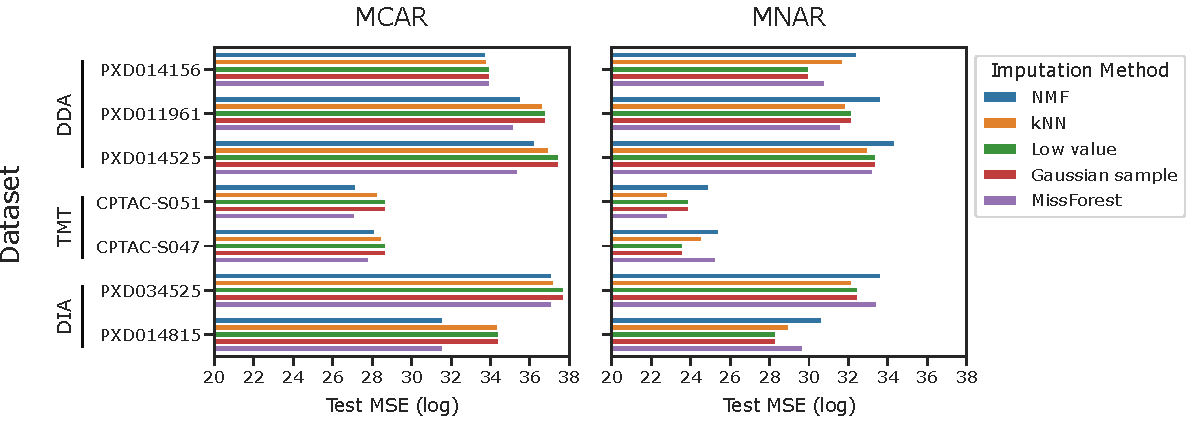
\includegraphics[width=0.95\textwidth]{figures/traditional-evaluation-figure.pdf}
  \caption{{\bf Evaluating imputation methods with traditional criteria.} 
  Test set reconstruction error (MSE) for imputation with five methods is shown, for seven proteomics data sets. MCAR and MNAR procedures were used to simulate missing values.}
  \label{fig:traditional-eval}
\end{figure}

Our results (Figure \ref{fig:traditional-eval}) demonstrate that the relative performance of imputation methods depends on the type of missingness. MissForest and NMF perform the best for all seven data sets in the MCAR condition. In the MNAR condition, the two single-value imputation methods---Gaussian sample and low value replacement---appear to work the best, though MissForest also performs well for some data sets. In both conditions, the two TMT data sets---CPTAC-S047 and CPTAC-S051---yield lower reconstruction errors across all imputation methods when compared to the DDA and DIA data sets. 

\subsection{Evaluating with downstream-centric criteria}

Although traditional machine learning-style evaluations such as Figure~\ref{fig:traditional-eval} are informative, we argue that prediction error on a held-out set is neither the most convincing nor the most relevant metric for most proteomics researchers. Additionally, good performance per traditional evaluation criteria may not translate to good performance on downstream analysis tasks. Furthermore, recent benchmarking studies have made the assumption that imputation will improve performance on downstream analysis tasks relative to no imputation. This assumption is generally unfounded, as imputation can introduce bias even when used appropriately \cite{scRNAseq-false-signals, sc-impute-gene-networks}. With these considerations in mind, we compared the performance of five commonly used imputation methods on three downstream analysis tasks that we argue are more congruent with the questions proteomicists typically seek to answer.

\subsubsection{Differential Expression}

We began with differential expression analysis. We obtained peptide-level quantifications from a DIA-based clinical study of Alzheimer's disease \cite{smtg-maccoss}. Patient-derived brain samples had been assigned to experimental groups based on several genetic, histopathological and cognitive criteria. We compared samples belonging to two experimental groups: (i) autosomal dominant dementia and (ii) high cognitive function, low Alzheimer's disease neuropathologic change. These experimental groups represent opposite ends of the spectrum of Alzheimer's disease severity and Merrihew \textit{et al.} found significant biological heterogeneity between them. 

\begin{figure}
  \centering
  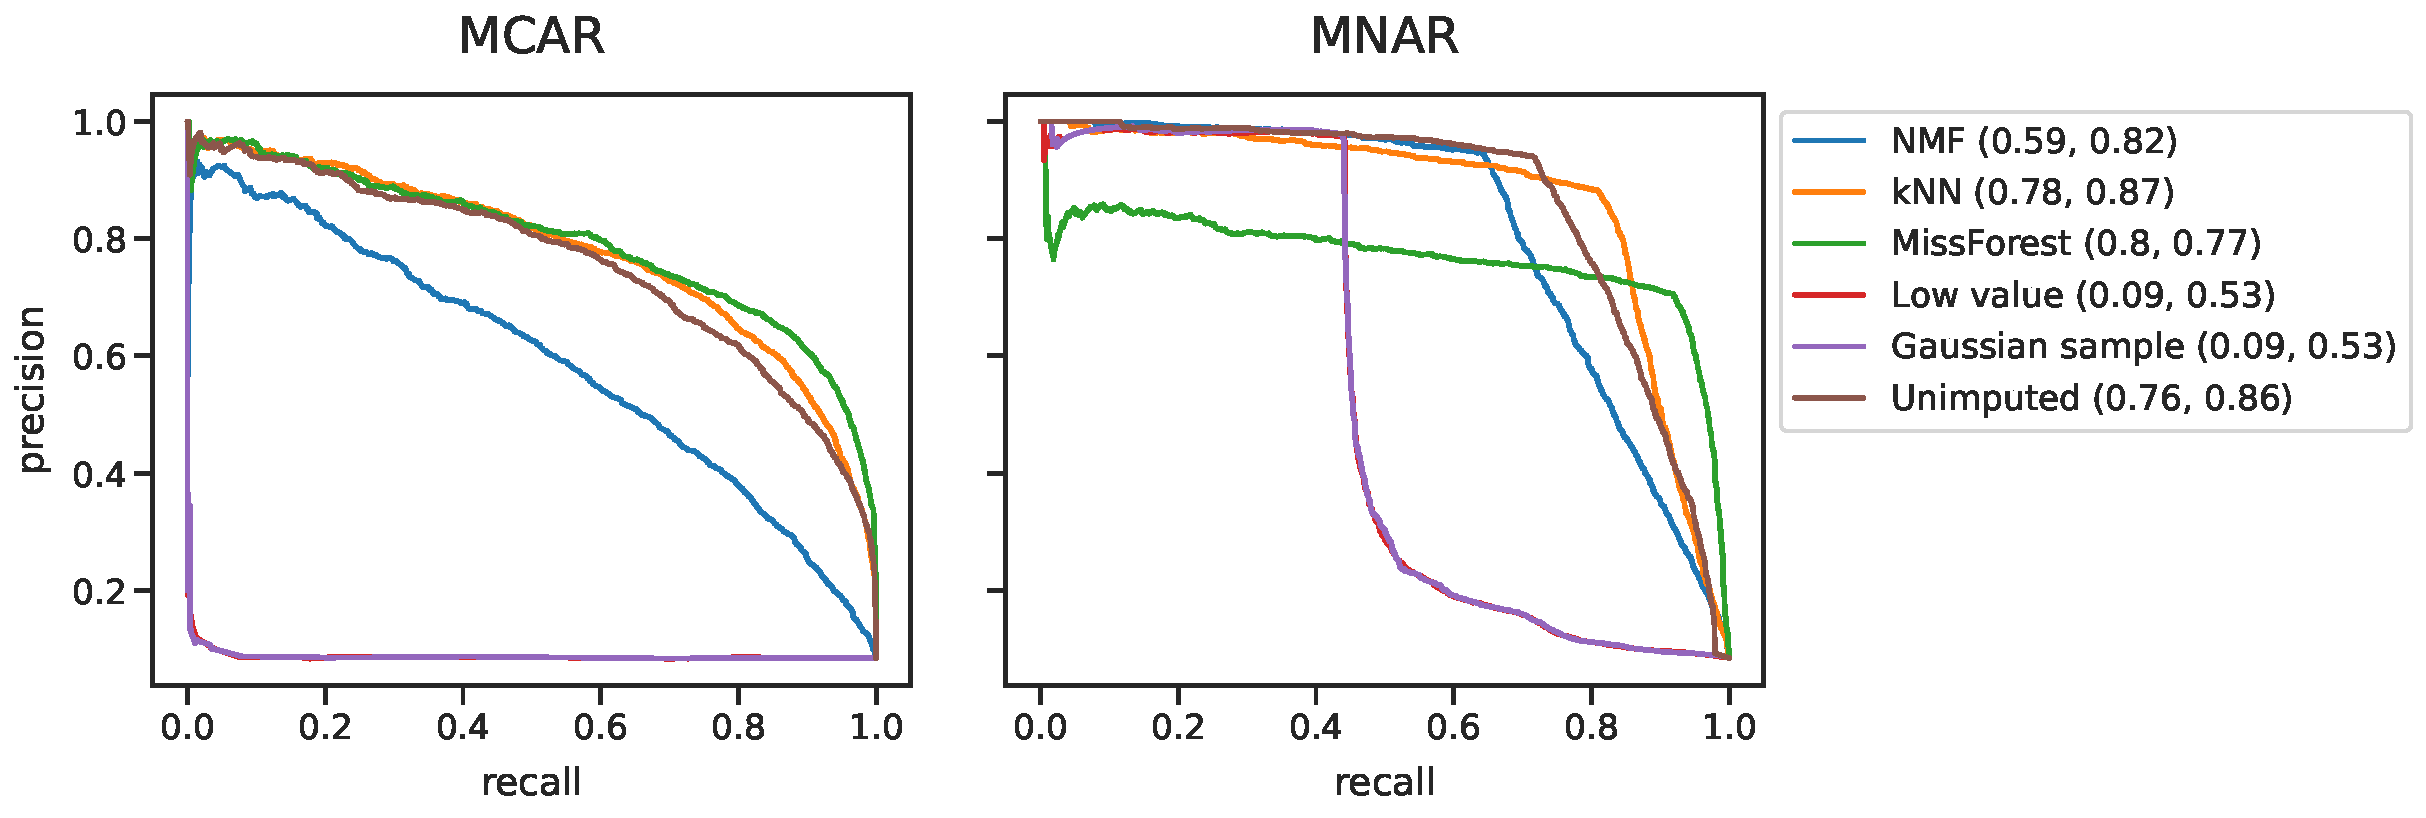
\includegraphics[width=1.0\textwidth]{figures/differential-expression-DIA-peptide-figure.pdf}
  \caption{{\bf Comparing the abilities of imputation methods to identify differentially expressed peptides.} Precision-recall curves are shown, for MCAR and MNAR simulated missingness. Data were obtained from PXD034525, a DIA study of Alzheimer's disease. Differentially expressed peptides were identified between two clinically annotated Alzheimer's disease groups \cite{smtg-maccoss}. The areas under the precision-recall curves (AUCs) for MCAR and MNAR are indicated.}
  \label{fig:PR-curves}
\end{figure}

\begin{figure}
  \centering
  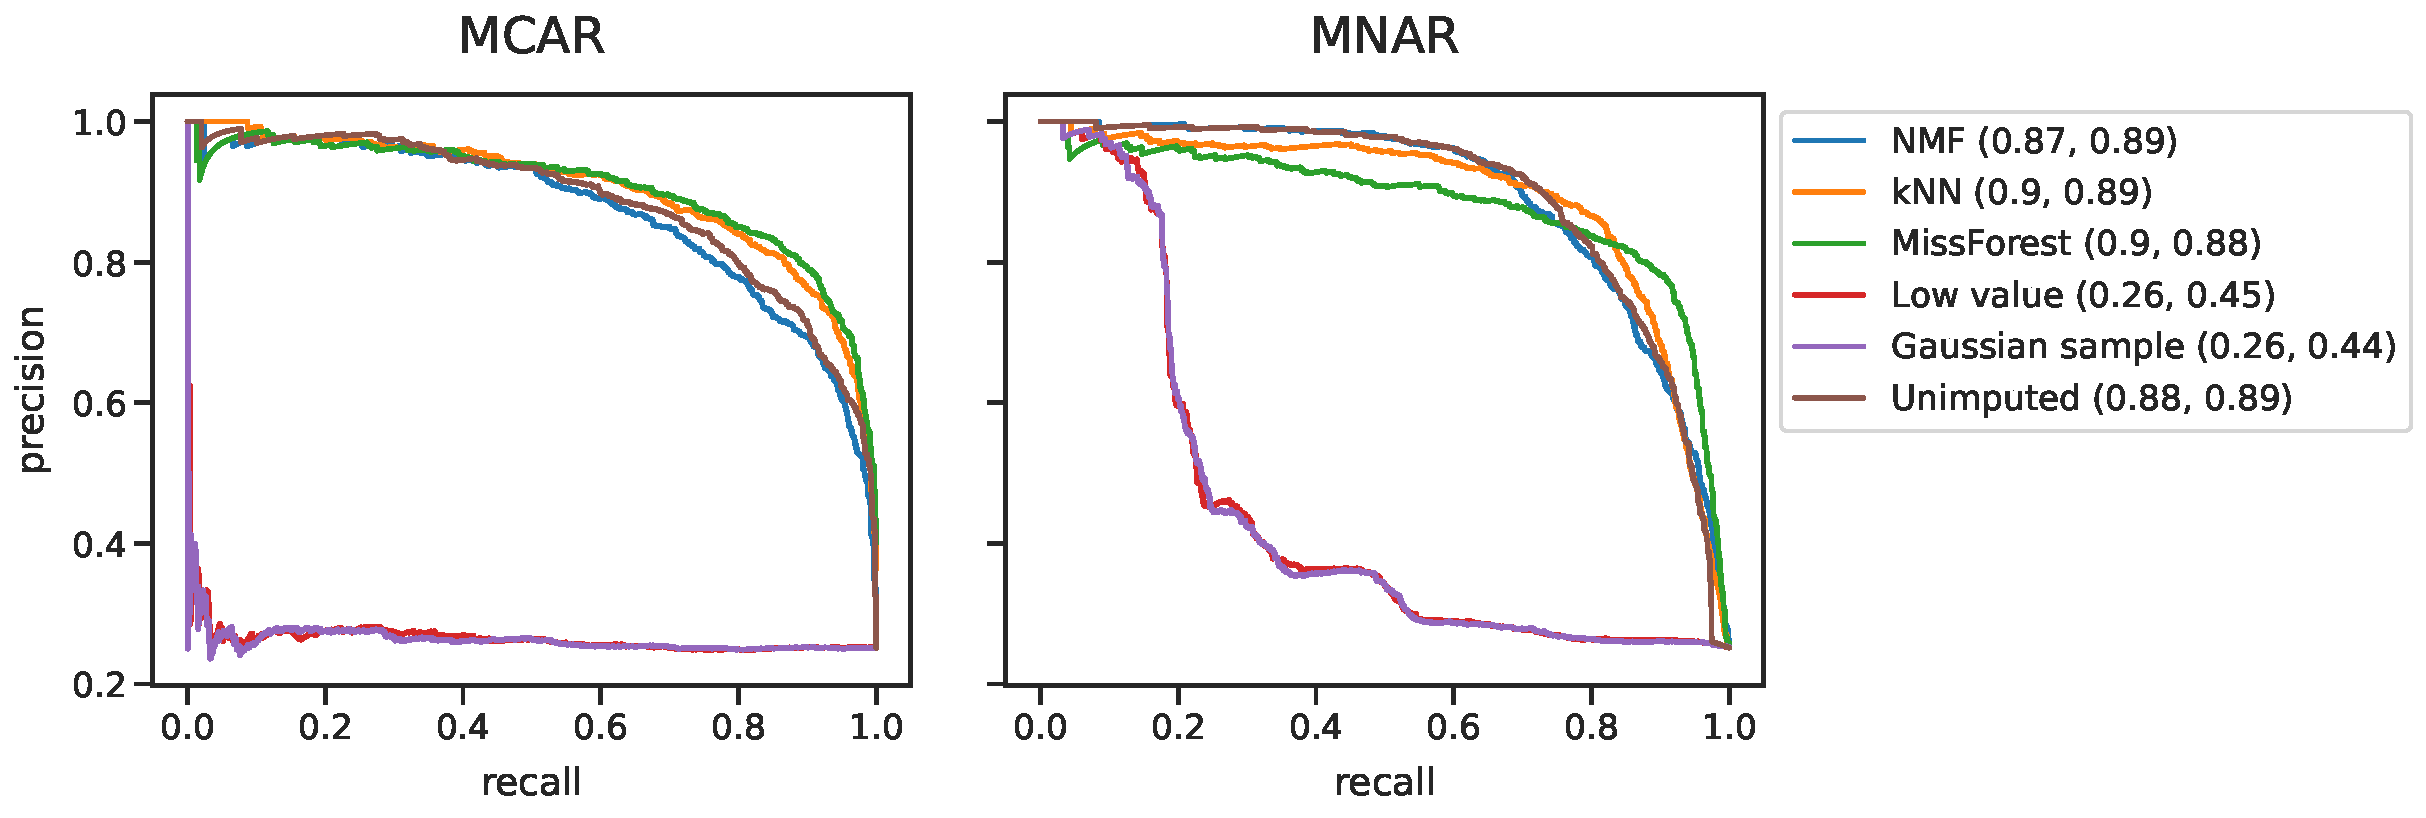
\includegraphics[width=1.0\textwidth]{figures/differential-expression-DIA-protein-figure.pdf}
  \caption{{\bf Comparing the abilities of imputation methods to identify differentially expressed proteins.} DIA data were obtained from PXD03452. Differentially expressed proteins were identified between two clinically annotated Alzheimer's disease groups. Missingness was simulated with MCAR and MNAR. AUC values are shown in parentheses.}
  \label{fig:PR-curves-protein}
\end{figure}
 
We compared the abilities of imputation methods to identify differentially expressed peptides after simulating missingness with either MCAR or MNAR (Figure~\ref{fig:PR-curves}). To perform this experiment, we identified ground truth differentially expressed peptides in the low-missingness Alzheimer's disease DIA data set, simulated 30\% missingness, then imputed with various methods and identified differentially expressed peptides in the imputed matrices. We also included an unimputed condition in which differentially expressed peptides were identified directly from the unimputed training set. The sharp elbows in the MNAR precision-recall curves are due to the fact that an alpha value of 0.01 was used for determining significantly differential peptides for both ground truth and imputed matrices. It is likely that many peptides had p-values very close to the 0.01 threshold but were not considered differentially expressed, resulting in sharp decreases in precision as soon as this threshold was crossed.

In the MCAR condition, MissForest, kNN and no imputation all performed well, with areas under the curve (AUCs) of 0.80, 0.78 and 0.76, respectively. In the MNAR condition, kNN, no imputation and NMF performed the best, with respective AUCs of 0.87, 0.86 and 0.82. While the two single-value imputation methods performed well in the MNAR condition of the traditional evaluation experiment (Figure \ref{fig:traditional-eval}), they performed poorly on the differential expression test, with the lowest AUCs for both MCAR and MNAR. In both conditions, no imputation performed nearly the same or better than the five imputation methods. 

We also performed differential expression experiments for a TMT (Supplementary Figure 3) and a label-free DDA (Supplementary Figure 4) data set. For the TMT data set, no imputation performed the best for MCAR, and was slightly outperformed by kNN for MNAR. For the label-free DDA data set, no imputation performed the best for both MCAR and MNAR. For the label-free DDA data set the single-value impute methods were the worst performing for both MCAR and MNAR.

We revisited the Alzheimer's disease DIA data set to perform a final differential expression experiment for \textit{protein-level} quantifications (Figure \ref{fig:PR-curves-protein}). In both MCAR and MNAR conditions, the single-value imputation strategies performed the worst. Interestingly, the AUCs of the non-single value imputation strategies were all in the range of 0.87--0.9. This indicates that, for this particular DIA data set, differential expression analysis was more accurate at the protein level. We again observed that no imputation performs remarkably well relative to commonly used imputation methods, with AUCs of 0.88 and 0.89 for MCAR and MNAR, respectively.

\subsubsection{Quantitative Peptides}

Next, we assessed whether imputation can generate additional quantitative peptides. While peptide detection rates have increased significantly over the past decade, not every detected peptide is necessarily quantitative. For a peptide to be considered quantitative, increases in measured signal must correspond to increases in peptide abundance, across a linear range \cite{matrix-matched-calib}. We obtained data from a serial dilution series experiment (PXD014815) in which the protein concentration was known for each sample. We used a statistical model developed by Pino \textit{et al.} to determine whether each detected peptide was quantitative before and after imputation \cite{matrix-matched-calib}.

\begin{figure}[t]
  \centering
  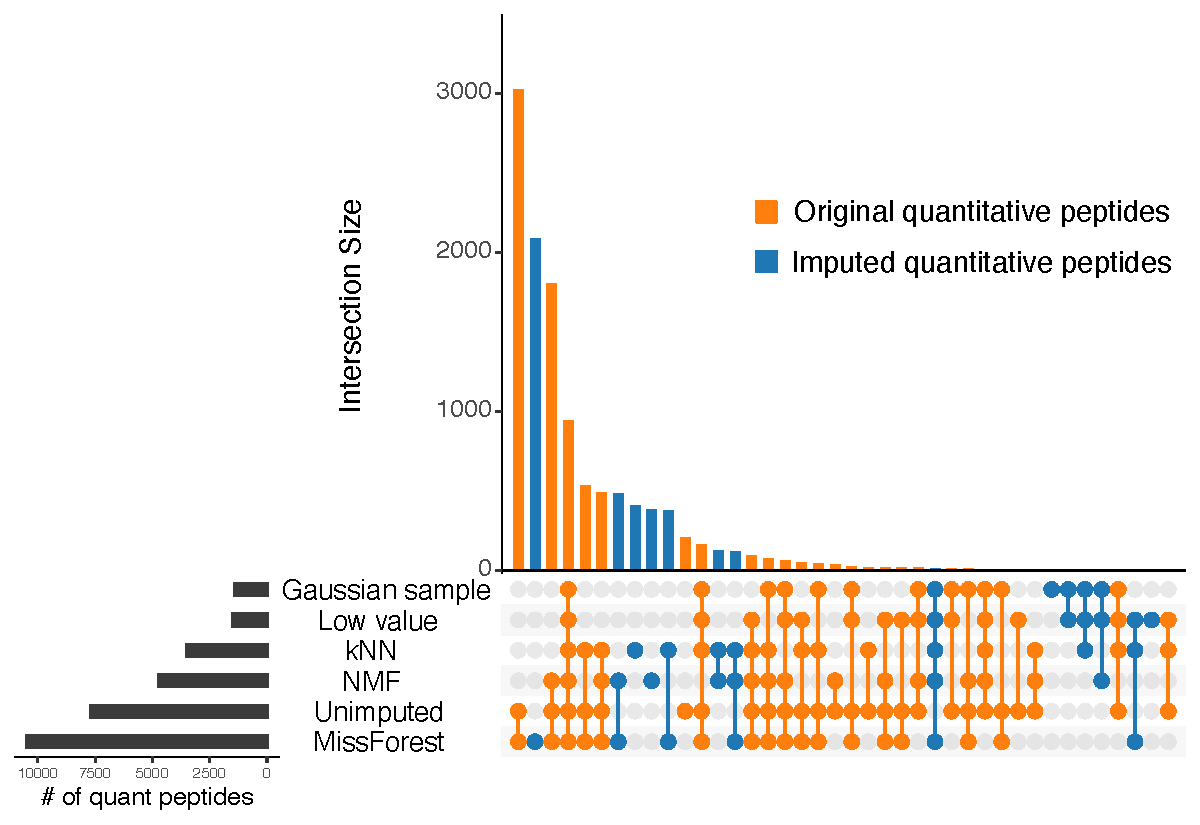
\includegraphics[width=0.9\textwidth]{figures/n-quant-peptides-figure.pdf}
  \caption{{\bf Comparing the abilities of imputation methods to generate additional quantitative peptides.} Orange indicates peptides that were quantitative in both the imputed and unimputed data sets. Blue indicates peptides that were only quantitative after imputation. Data were obtained from PXD014815 \cite{matrix-matched-calib}.}
  \label{fig:rescue-experiment}
\end{figure}

The results of this experiment (Figure \ref{fig:rescue-experiment}) show that several imputation methods produce new quantitative peptides. MissForest, kNN and NMF each generated large sets of peptides that were quantitative only after imputation (2,768 for MissForest; 1,050 for kNN; 1,128 for NMF). However, MissForest was the only method that increased the \textit{total} number of quantitative peptides relative to no imputation, producing 10,475 quantitative peptides relative to the 7,707 obtained with no imputation. 

\subsubsection{Lower limit of quantification}

We also assessed whether imputation can improve peptide LLOQ, which refers to the minimum abundance at which a peptide can be considered quantitative. For this analysis, we again used the serial dilution data set from Pino \textit{et al.}. We found that while imputation did indeed decrease the LLOQ for many peptides, it also \textit{increased} the LLOQ for some peptides, which was the opposite of the intended effect. Strikingly, MissForest was the only method that decreased the LLOQ of significantly more peptides than it increased (Figure \ref{fig:lloq}, one-sided binomial p-value corrected with Benjamini-Hochberg $<$ 0.01).

\begin{figure}
  \centering
  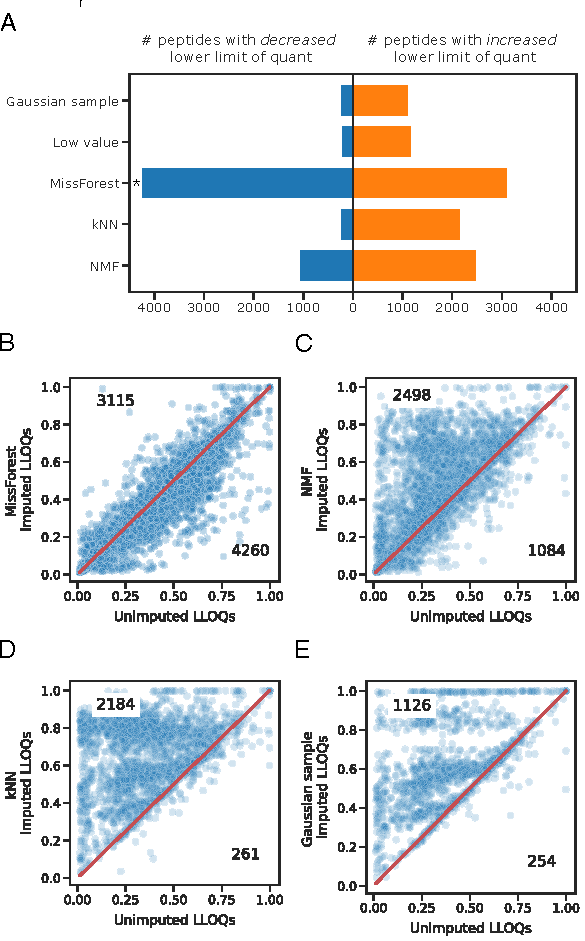
\includegraphics[width=0.7\textwidth]{figures/lloqs-figure.pdf}
  \caption{{\bf Comparing the abilities of imputation methods to decrease peptide LLOQ.}  In (A) the asterisk indicates a one-sided binomial Benjamini-Hochberg corrected p-value $<$0.01. In (B--E) the LLOQs of unimputed peptides are plotted against the LLOQs of the same imputed peptides. Only peptides with changes in LLOQ following imputation are plotted. Data were obtained from PXD014815 \cite{matrix-matched-calib}.}
  \label{fig:lloq}
\end{figure}

\subsection{Runtime}

For imputation methods to be incorporated into existing proteomics data processing workflows, they must be runnable in a reasonable time frame. With this in mind, we compared the runtimes of our five imputation methods (Figure \ref{fig:runtime}). The two simplest methods, Gaussian sample and low value replacement, ran in a matter of seconds; NMF and kNN ran in a matter of minutes; MissForest took several hours to complete. Thus, with the possible exception of MissForest, runtime should not present a barrier for incorporation into data processing workflows.

\begin{figure}
  \centering
  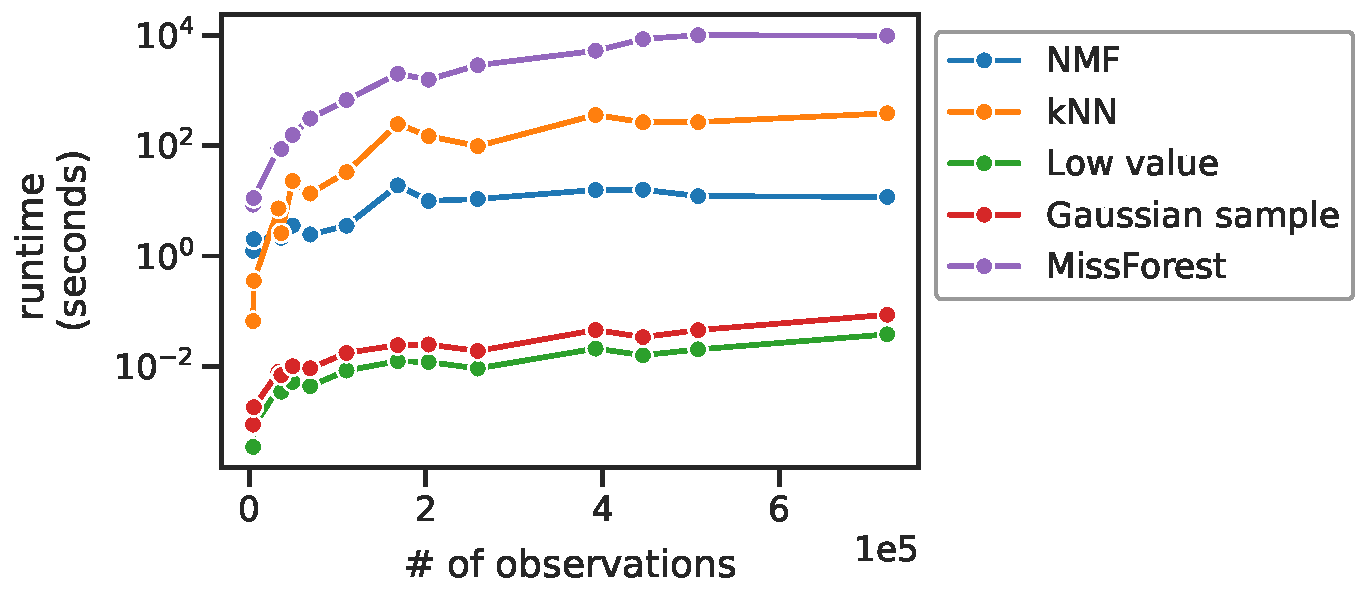
\includegraphics[width=0.8\textwidth]{figures/runtimes-figure.pdf}
  \caption{{\bf Runtime comparison for imputation methods.} Each point represents a data set. Data sets are ordered by the number of non-missing observations in their training sets after an 80\%/20\% MCAR train/test partition.}
  \label{fig:runtime}
\end{figure} 

\subsection{Variance in quantitative proteomics data}

We investigated the statistical assumptions underlying several imputation approaches. Peptide quantifications are often assumed to be Poisson distributed, while log transformed quantifications are assumed to be Gaussian \cite{ms-dist-derivation, stat-theory-lcms, kimmel-2005}. A feature of a Poisson distribution is that variance is equivalent to the mean, while for a Gaussian distribution variance is constant. Parametric imputation methods with a Gaussian prior include least-squares regression, the Gaussian sample impute method, and standard NMF.

To empirically investigate the variance of peptide quantifications, we obtained data from four experiments, each of which contained technical replicates (Table \ref{tab:data-description}). We used three DDA experiments and one DIA. We calculated the means and variances of peptide quantifications across technical replicates, for each detected peptide, for each experiment. We found that peptide quantifications are overdispersed relative to the Poisson distribution (Figure \ref{fig:mean-x-var}, left); that is, for nearly every peptide, the variance across replicates was greater than the mean intensity across replicates. Log transformation resulted in more uniform variance across intensities, but many peptides still displayed extraordinarily high variances (Figure \ref{fig:mean-x-var}, right). 

We found that for multiple data sets obtained with both DDA and DIA acquisition strategies, neither Poisson nor Gaussian assumptions hold. This suggests that parametric imputation methods with implicit Gaussian assumptions may be ill-suited for these data. 

We also observed that imputation with NMF and MissForest had little effect on the variance of peptide quantifications (Supplementary Figure 5). The Gaussian sample method, however, introduced additional variance. This finding suggests that while NMF and MissForest imputation do not profoundly affect the underlying distribution of peptide quantifications, single-value impute strategies may do so. In this way, single-value impute strategies may introduce artifacts into proteomics data when their underlying assumptions are not met.

\begin{figure}
  \centering
  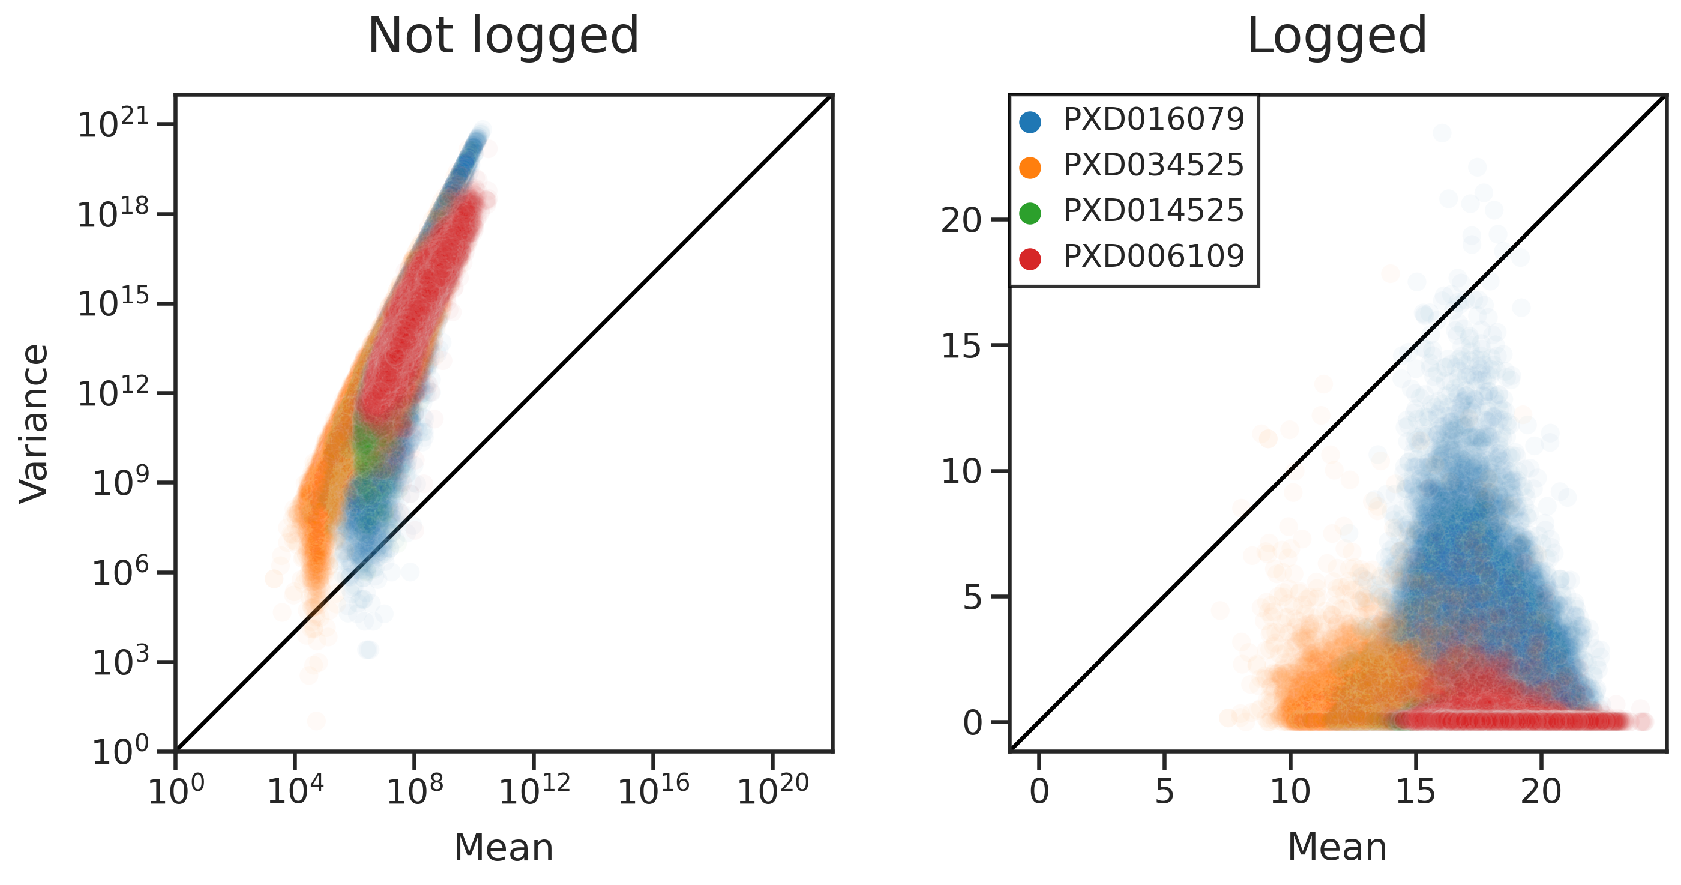
\includegraphics[width=0.65\textwidth]{figures/mean-variance-peptide-figure.pdf}
  \caption{{\bf Variance of peptide quantifications is greater than expected.} Means and variances were calculated across technical replicates for every detected peptide. Each dot corresponds to a peptide. Data from DIA (PXD034525) and DDA (PXD016079, PXD014525, PXD006109) experiments are plotted.}
  \label{fig:mean-x-var}
\end{figure} 

\section{DISCUSSION}

The two most popular imputation methods---Gaussian sampling and low value replacement---performed poorly in our downstream-centric experiments. These single-value imputation strategies were the worst perfoming for peptide-level differential expression detection in DIA data (Figure \ref{fig:PR-curves}), protein-level differential expression in DIA data (Figure \ref{fig:PR-curves-protein}), peptide-level differential expression in label-free DDA data (Supplementary Figure 4), generating quantitative peptides (Figure \ref{fig:rescue-experiment}) and decreasing peptide LLOQ (Figure \ref{fig:lloq}). 

However, the results of the downstream-centric experiments did not always agree with the traditional evaluation experiment. In particular, the single-value imputation strategies often outperformed the local and global similarity strategies for the traditional benchmarking experiment shown in Figure \ref{fig:traditional-eval}, especially for MNAR. This was likely because the single-value imputation strategies assume that missing values are drawn from the low end of the distribution of peptide quantifications, and this assumption was met in the MNAR condition of the traditional evaluation experiment. We argue that traditional evaluation experiments such as Figure \ref{fig:traditional-eval} are misleading because they inflate the performance of single-value impute strategies. Performance on our downstream-centric criteria is more relevant than test set MSE, because the downstream criteria are more congruent with questions proteomics researchers typically seek to answer. Thus, we urge the community to move away from traditional performance evaluations in favor of the downstream-centric criteria presented here.

Our results suggest that imputation may not be necessary for differential expression analysis. For a DIA experiment with MCAR and MNAR simulated missingness, no imputation worked roughly as well as the best imputation methods (Figure \ref{fig:PR-curves}). In the MCAR condition, the largest AUC value belonged to MissForest at 0.8, only slightly higher than unimputed at 0.76. In the MNAR condition, kNN had the highest AUC at 0.87, and unimputed was close behind with 0.86. This result generalized to a label-free DDA data set (Supplementary Figure 4), in which no imputation outperformed all imputation methods for MCAR and MNAR. For a TMT data set, no imputation had the highest AUC for MCAR and was tied for the second highest for MNAR (Supplementary Figure 3).

We found that as the missingness fraction increased, unimputed performed better and better relative to the five imputation methods (Supplementary Figure 2). For example, in the case of MNAR with a 50\% missingness fraction, unimputed had an AUC of 0.65, whereas the best imputation method was MissForest with an AUC of 0.55. 

We also found that for a DIA experiment, differential expression analysis was more accurate when performed at the protein level (Figure 4). This makes sense because protein roll-up reduces missingness and hides variability between peptides of the same protein, therefore making the differential expression identification task easier \cite{humpty-dumpty}.
Researchers should approach protein-level analysis with caution, however, because protein roll-up may introduce statistical bias and reduce data heterogeneity \cite{humpty-dumpty, boekweg-2023}. It should be noted that once again, the unimputed condition had one of the highest AUC values for both MCAR and MNAR.

Taken together, our differential expression results cast doubt on the practice of imputing missing values prior to differential expression analysis. We have shown that at the peptide and protein level, for DIA, label-free DDA and TMT experiments, no imputation generally works as well as the most commonly used imputation methods. Our results are in line with Wolski \textit{et al.}, who suggest that statistical models of differential expression that do not impute, but rather explicitly model missingness, tend to outperform traditional models \cite{prolfqua}.

As we only performed differential expression analysis on three data sets, we do not claim our results will generalize to all proteomics data. Instead, our results suggest that researchers should empirically evaluate whether imputation improves accuracy of their differential expression analysis on a case-by-case basis, using similar procedures to the one we introduce here.

Bai \textit{et al.}\ have shown that the choices in normalization procedure and statistical analysis method can affect differential expression results \cite{bai-2023}. The normalization procedures used by the data sets we analyzed are provided as Supplementary Table 1. We acknowledge that differences in normalization may have introduced variation that cannot be explained by the imputation methods alone. It is also possible that the spectral processing tools themselves---for example MaxQuant versus Skyline---may have contributed additional variation. Future work will aim to repeat our benchmarking analysis with standardized spectral processing and normalization procedures.

We choose a two-sample sample t-test for differential expression analysis because it represents a simple, transparent and commonly used procedure\cite{brunner-2022, pxd007683, pxd006348, pxd016079}. Furthermore, the three data sets we analyzed all had relatively simple experimental designs. For the DIA\cite{smtg-maccoss} and TMT\cite{CPTAC-S047} data sets, each analyzed sample came from a different individual, and serial biopsies and time series data were excluded from our analysis. For the label-free DDA data set\cite{pxd006348}, biological replicates from two \textit{Brucella} species were compared. For simple experimental designs such as these, differential expression analysis does not require complicated statistical procedures. 
For more complex designs we recommend MSstats, which can model a variety of experimental designs in a statistically rigorous manner\cite{ms-stats}.

We found that imputation can identify new quantitative peptides (Figure \ref{fig:rescue-experiment}). As modern proteomics techniques increase the number of identifications, it is important to remember that not all detected peptides are quantitative. Here we show that MissForest can be used as a post-processing tool to generate additional quantitative peptides in a proteomics experiment (Figure \ref{fig:rescue-experiment}). Additionally, NMF and kNN can produce new subsets of quantitative peptides, even though they may still decrease the total number of quantitative peptides. Increasing the number of quantitative peptides will increase the statistical power of any downstream prediction or inference task that relies on peptide abundances. Such tasks include identifying differentially expressed peptides, clustering samples or peptides, dimensionality reduction and identifying co-expression modules and protein-protein interaction networks.

Imputation with MissForest can also improve peptide LLOQ (Figure \ref{fig:lloq}). It is worth acknowledging that while MissForest decreased the LLOQ of significantly more peptides than it increased, it did still increase the LLOQ for a large number of peptides (3,115/24,204 detected peptides). That said, any proteomics study that examines biologically important low-abundance peptides may still benefit from MissForest imputation. As the scale and sensitivity of proteomics experiments increase, MissForest---and future imputation methods---may help researchers study key peptides derived from ever-smaller sample volumes. 

Finally, we provide empirical evidence that peptide quantifications exhibit more variance than can be explained under Poisson or Gaussian modeling assumptions (Figure \ref{fig:mean-x-var}). While ion counting may be a Poisson process \cite{ms-dist-derivation, stat-theory-lcms, kimmel-2005}, it is clear that the resulting quantifications are not Poisson distributed. One property of a Poisson distribution is that mean and variance are equal. We found that this property was violated by several proteomics data sets: the variance among peptide quantifications across technical replicates was greater than the corresponding means (Figure \ref{fig:mean-x-var}). This result held true for both DDA and DIA experiments and for protein-level quantifications (Supplementary Figure 6). We speculate that this additional variance may be due to an unaccounted-for noise source such as electrospray ionization. Another assumption is that log-transformed intensities are roughly Gaussian. Under this model, variance would be uniform across mean intensities. We show this assumption is also violated in DIA and DDA data: we observed non-uniform variance after log transformation (Figure \ref{fig:mean-x-var}, right).

Future imputation methods should explicitly model the variance present in proteomics data. One obvious choice of generating distribution is the negative binomial distribution, which has an additional parameter that can account for variance independent of the mean. This strategy has been employed previously to model counts from single-cell RNA sequencing experiments \cite{ZINB, neg-binom-scRNAseq}. Another option could be to perform variance stabilization prior to imputation. This is the goal with the log transformation; however, as we have shown, logging does not successfully stabilize variance. VSN, a custom variance stabilizing transformation originally developed for microarrays, has been shown to stabilize the variance of protein quantifications \cite{variance-stable-microarray, valikangas}, as has the generalized log transformation \cite{ms-noise-2-component}. However, the proteomics community is yet to broadly adopt these methods. Proteomics may also benefit from the variance stabilization technique developed by Bayat \textit{et al.}, in which a variance stabilizing function is empirically learned from the data \cite{variance-stable}. Successful modeling and variance stabilization approaches could benefit not just imputation but data analysis for proteomics more broadly.

We speculate that the unusual dimensionality of peptide-by-run matrices, generally thousands of peptides by less than 100 runs, may cause problems for existing imputation methods. Many proteomics imputation methods were originally developed for microarrays and relatively square matrices. Future imputation methods may benefit from explicitly accounting for the dimensionality of peptide-by-run matrices. 

The proteomics community would benefit from easy-to-use and broadly applicable imputation methods. As previously reported \cite{Bramer:review, Webb-Robertson:review, DIMA, lazar}, we found that the best choice in imputation method depends on the analysis task and the details of the experiment. This suggests the need for new imputation methods that are generalizable enough to accurately handle data from any acquisition strategy and type of missingness. Deep neural networks have proven highly generalizable in other contexts. Recent ``deep'' impute methods may be a step in the right direction \cite{deep-impute}, though much work remains to be done. In the future, data-driven imputation methods may be broadly adopted as part of general signal processing workflows for proteomics.

\section*{ASSOCIATED CONTENT}
\subsection*{Data Availability Statement}
The code used to generate all the figures in this manuscript can be found at:
\url{https://github.com/Noble-Lab/2023-prot-impute-benchmark}. The custom NMF imputation model can be found at \url{https://github.com/Noble-Lab/MSFactor}. All data sets used in this study are publicly available and can be found on PRIDE, CPTAC or Panorama \cite{PRIDE, CPTAC, panorama-public}. In addition, Data 1 provides the full results of our literatures search, including names and DOIs of the identified studies, and Data 2 provides a complete list of file names obtained for each PRIDE, CPTAC and Panorama experiment. Data 1 and 2 can be found at:
\url{https://github.com/Noble-Lab/2023-prot-impute-benchmark/tree/main/supplemental}.

\subsection*{Supporting Information}
The Supporting Information is available free of charge at \fixme{xxx}.

\section*{ACKNOWLEDGMENTS}
The authors thank Michael J.\ MacCoss of the University of Washington's Department of Genome Sciences for helpful discussions. This work was supported by National Institute on Aging grant number 1F31AG082395-01.

\section*{AUTHOR INFORMATION}
\textbf{Corresponding Author} \\
William S.\ Noble, email: william-noble@uw.edu

\textbf{ORCID} \\
Lincoln Harris: 0000-0003-2544-4225 \\
William E.\ Fondrie: 0000-0002-1554-3716 \\
Sewoong Oh: 0000-0002-8975-8306 \\
William S.\ Noble: 0000-0001-7283-4715

\textbf{Notes} \\
The authors declare no competing financial interests.

\bibliographystyle{unsrt}
\bibliography{references.bib} 

\end{document}
